\chapter{Networking e Sicurezza}

Il mondo embedded e IoT in questi anni sta avendo un forte sviluppo, grazie alla disponibilità di dispositivi dal rapporto prestazioni/prezzo vantaggioso, e ha creato un grande bacino di utenza di esperti, o semplici neofiti, interessati al mondo dell'elettronica/informatica dedicata. Un effetto positivo di questa evoluzione è lo sviluppo di librerie open-source e di sistemi software orientati all'IoT.

Questo trend ha creato un mercato sempre più vasto di produttori di dispositivi più performanti, economici e dalle dimensioni ridotte (perfetti per realizzazioni embedded).
A causa di questo sviluppo, per certi versi incontrollato, "tutto" è virtualmente collegato/collegabile \textit{online} e sembra essere passata in secondo piano la progettazione di hardware e software che tiene conto della \textbf{sicurezza dei sistemi}. I primi attacchi mirati a queste tecnologie hanno avuto facilità di esecuzione e una rapidissima diffusione\footnote{Breve lista di attacchi a sistemi IoT nel 2015 \url{http://tinyurl.com/honlko2}.}.

In questo scenario, dalla parte dei produttori hardware si registra una mancanza o addirittura una resistenza per quanto riguarda la correzione di falle o il rilascio di aggiornamenti firmware. Questo potrebbe essere dovuto all'utilizzo di codice proprietario o la totale mancanza di supporto per il dispositivo che si utilizza. In alcuni casi si potrebbe parlare di \textbf{obsolescenza programmata}\footnote{Obsolescenza programmata - \url{https://it.wikipedia.org/wiki/Obsolescenza_programmata.}}.

Anche da parte degli utilizzatori finali dei sistemi non si evince una particolare attenzione ai problemi relativi alla sicurezza; probabilmente a causa delle scarse conoscenze del sistema in uso (perché complesso o non studiato) e delle tecnologie usate. È ormai tristemente noto che lo sviluppo di questi \textbf{\textit{dispositivi perennemente connessi}}, non prende quasi mai in considerazione le problematiche relative alla sicurezza derivata dalla connessione a sistemi più \textit{fragili} o legate all'interazione con altri device (perdita di privacy, prestazioni o utilizzo improprio di risorse di rete).\\

Jimmy Challenge è stato sviluppato garantendo la sicurezza del sistema e dei giocatori.\\

In questo capitolo verranno presentate alcune delle soluzioni adottate e delle tecnologie utilizzate per l'implementazione dell'applicativo lato server e dei collegamenti di reti.
Per scelta progettuale ed etica, ove possibile, si è preferito utilizzare esclusivamente software \textit{open-source}.

\subsection{Sistema Operativo}
Le mansioni di server sono fisicamente compiute da un \textbf{Odroid C2}) il quale utilizza come OS una versione ARM a 64-bit della distribuzione Linux \textbf{Arch Linux ARM}.

\subsubsection{Arch Linux ARM} 
\begin{itemize}
	\item è \textit{bleeding edge} per quanto riguarda l'upstream degli aggiornamenti (sempre aggiornata all'ultima versione dei software disponibile);
	\item generalmente è considerata sicura;
	\item fornisce una libertà maggiore per la configurazione del sistema;
	\item una forte e grande community.
\end{itemize}

\subsubsection{Software installato orientato alla sicurezza}
\begin{itemize}
	\item \textbf{SSH} con autenticazione chiave pubblica-privata RSA;
	\item firewall \textbf{UFW}, per rendere disponibili all'esterno soltanto alcuni servizi;
	\begin{itemize}
		\item 80: Web Server;
		\item 22: SSH;
		\item 443: HTTPS.
	\end{itemize}
	\item \href{https://certbot.eff.org/}{Cerbot} per i certificati SSL/TLS;
	\item\href{https://github.com/firehol/netdata}{Netdata}  per una visualizzazione delle risorse del sistema da remoto.
\end{itemize}
Oltre all'installazione e alla configurazione dei software sono stati configurati diversi parametri per l'\textit{hardening} del kernel tramite \textit{sysctl} ed un sistema di \textit{logging} per la registrazione degli accessi.

\subsection{NGINX e HTTPS}
\textbf{NGINX} è un web server orientato alle performance, al ridotto consumo di risorse e alla facilità di configurazione.
In un sistema come l'Odroid con potenza computazionale ridotta (rispetto ai classici server) l'utilizzo di applicativi con ridotto consumo di risorse garantisce una maggiore reattività del sistema e un migliore risultato agli occhi dell'utente.

La configurazione di NGINX prende in considerazione tutti i maggiori problemi legati all'esposizione di un sito e di un web server in rete: buffer overflow, DDoS, bruteforcing, sniffing, etc. e cerca di mitigare o prevenire ogni tipo di attacco senza generare intralcio o rallentamenti all'utilizzo standard del web server.\\
Grazie a \textit{Cerbot} è possibile ottenere certificati SSL/TLS gratuitamente e garantire un canale di comunicazione protetto tra client e server.\\
La configurazione di NGINX è visibile \href{https://raw.githubusercontent.com/FedericoTorsello/Embedded/serverPHP/nginx.conf}{qui}.\\
L'intera configurazione di NGINX cerca di essere compatibile con gli ultimi protocolli e limitare quelli obsoleti e poco sicuri, rischiando però di ridurre la compatibilità con i browser minori. Per garantire ulteriori performance NGINX è abilitato ad instaurare connessioni tramite il recente protocollo HTTP/2 con i client compatibili.

\subsection{MySQL, Redis}
MySQL e Redis:
\begin{itemize}
	\item non sono esposti verso l'esterno;
	\item sono protetti da password;
	\item sono configurati per rispettare il POLP (\textit{principle of least privilege}).
\end{itemize}
\subsubsection{MySQL}
Con \textbf{MySQL} si gestisce il database per lo storage delle credenziali degli utenti e la lista degli utenti connessi online.
\begin{lstlisting}[frame=none]
CREATE TABLE IF NOT EXISTS users (
id int(3) NOT NULL AUTO_INCREMENT PRIMARY KEY,
created DATETIME DEFAULT CURRENT_TIMESTAMP,
username varchar(15) COLLATE utf8_general_ci NOT NULL,
password varchar(255) COLLATE utf8_general_ci NOT NULL,
email varchar(30) COLLATE utf8_general_ci NOT NULL,
keepalive DATETIME DEFAULT CURRENT_TIMESTAMP ON UPDATE CURRENT_TIMESTAMP,
logged boolean NOT NULL DEFAULT 0,
) ENGINE=InnoDB DEFAULT CHARSET=utf8 COLLATE=utf8_general_ci;

ALTER TABLE users ADD INDEX logged_index(logged);

SET GLOBAL event_scheduler = ON;

DELIMITER $$
CREATE EVENT IF NOT EXISTS `keepalive_logged`
ON SCHEDULE EVERY 1 MINUTE STARTS '2016-06-01 00:00:00'
ON COMPLETION PRESERVE
DO BEGIN
UPDATE users SET logged = 0
WHERE TIMESTAMPDIFF(SECOND, keepalive, now()) >= 20;
END;$$
DELIMITER ;
\end{lstlisting}
Un event MySQL controlla periodicamente se un utente è ancora collegato o meno.

\subsubsection{Redis}
\textbf{Redis} è un applicativo per lo store di strutture dati chiave-valore in memoria. Il principale vantaggio di Redis è la sua velocità in lettura e scrittura e la facilità di utilizzo.

\subsection{Sito Web, back-end e API RESTful}
Il sito web (sia front-end che back-end) è stato sviluppato tenendo a mente le linee guida del W3C e del OWASP.

Al fine di rendere l'applicativo il più possibile portabile, sono state implementate delle API RESTful in PHP7; sia l'applicativo Python lato client, sia il sito web (tramite AJAX) utilizzano queste API.

Una volta che un utente si è loggato, gli viene assegnato un \textit{token} JWS (JSON Web Signature) che deve essere validato ad ogni richiesta che farà da quel momento in poi. Questo token permette di verificare l'identità dell'utente ad ogni richiesta ed evitare usi improri della API da utenti malintenzionati.
Le API possono essere invocate solo tramite richieste POST e comunicano tramite messaggi JSON appositamente formattati.

In seguito al login effettuato, il sito web si presenta all'utente come un'unica pagina in cui è possibile inviare messaggi a tutti gli altri utenti collegati tramite una chat globale e selezionare un giocatore da sfidare. 

Una volta iniziata una partita, nella view principale della pagina appariranno i dati relativi allo stato della partita dell'avversario. Ogni aggiornamento dello stato verso i client è effettuato tramite Server-Sent Events (SSE).

Grazie a SSE, per mezzo del pattern \textbf{publish-subscribe}:
\begin{itemize}
	\item si riducono i consumi di risorse computazionali
	\item si limita l'utilizzo della banda
	\item si eliminano i problemi di gestione di altre tecnologie come WebSocket o WebRTC.
\end{itemize} 
Per farlo si instaura un canale mono direzionale verso il client in cui è possibile istruire il browser per controllare periodicamente l'aggioranemto dello stato dei dati o forzare l'invio di dati aggioranti da parte del server.

Per il back-end sono state utilizzate diverse librerie per fornire alcune funzionalità come JWS e SSE scelte appositamente per la loro compatibilità con gli ultimi standard e versioni di PHP al fine di garantire maggiori performance e sicurezza:
\begin{itemize}
	\item \href{https://github.com/namshi/jose}{jose}: per i token JWS;
	\item \href{https://github.com/licson0729/libSSE-php}{libSSE-php}: per SSE;
	\item \href{https://github.com/symfony/http-foundation}{http-foundation} e \href{https://github.com/nrk/predis}{predis}: come dipendenze di "libSSE-php".
\end{itemize}
Le interazioni tramite il database MySQL avvengono per mezzo di una connessione locale, utilizzando le varie tecniche di mitigazione per SQLi di primo e secondo livello fornite dal PHP.

Per proteggere la privacy degli utenti, le password sono salvate sul database come hash (usando bcrypt).

\subsection{Python}
Come anticipato nella relazione, per poter inviare al server i dati letti dalla seriale di Arduino è stato sviluppato uno script Python, in particolare \textbf{Python 3.5}.

\begin{figure}[!ht]
	\centering
	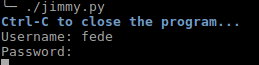
\includegraphics[scale=.8]{img/py.png}
	\caption{Login da terminale - lato client}\label{img:pythonTerminale}
\end{figure}

Tenendo a mente la visione dei sistemi embedded, dalle capacità computazionali ridotte rispetto ad un laptop o ad un PC desktop, si è deciso di utilizzare:
\begin{itemize}
	\item \href{https://github.com/pyserial/pyserial}{pyserial} : per la lettura dei dati dalla seriale;
	\item \href{https://github.com/pyserial/pyserial}{ujson}: per i messaggi JSON;
	\item \href{https://github.com/python/asyncio}{asyncio} : per eseguire le routine in maniera asincrona;
	\item \href{https://github.com/KeepSafe/aiohttp}{aiohttp}: come HTTP client per asyncio.
\end{itemize}
Per poter utilizzare lo script è necessario autenticarsi e ricevere il token JWS al fine di effettuare le richieste HTTP.

\subsubsection{Pyserial}
La libreria \textbf{pyserial} consente la connessione all'Arduino tramite porta seriale e la lettura dei messaggi in maniera continua grazie all'utilizzo di un thread che agisce da produttore di messaggi per l'intero script.

L'elaborazione di questi messaggi viene effettuata da una routine che dopo aver decodificato il messaggio lo instrada al corretto destinatario. Se si deve inviare un messaggio al server, viene composto il messaggio in JSON e viene inviato tramite una richiesta HTTP POST al server.

\subsubsection{Asyncio}
A parte il thread creato per la lettura dei messaggi da Arduino, le altre \textit{routine}, o meglio, \textit{\textbf{coroutine}} sono eseguite all'interno dell'event loop di asyncio. 

Asyncio fornisce una infrastruttura single-threaded per la scrittura di codice concorrente utilizzando coroutine, in particolare è consigliato per \textbf{programmi concorrenti IO-bound}. 

\subsubsection{Aiohttp}
Aiohttp fornisce un supporto per richieste HTTP asincrone tramite l'infrastruttura messa a disposizione da asyncio.

Questo tipo di approccio:
\begin{itemize}
	\item permette di ridurre i consumi di risorse;
	\item aumentare le performance dell'applicazione.
\end{itemize}
Questo risultato si ottiene perché la maggior parte dell'esecuzione dello script è basata sull'invio di dati al server.\\\\
L'obiettivo di rendere completamente asincrono il codice ed eliminare il thread della libreria \textit{pyserial} sarebbe possibile utilizzando delle API per \textit{asyncio} che sono però ancora incomplete ed non affidabili.